\documentclass[a4paper, 11pt]{article}
\usepackage{comment} % enables the use of multi-line comments (\ifx \fi) 
\usepackage{lipsum} %This package just generates Lorem Ipsum filler text. 
\usepackage{fullpage} % changes the margin
\usepackage{hyperref}
\usepackage{graphicx}

\begin{document}
%Header-Make sure you update this information!!!!
\noindent
\large\textbf{Assignment 9} \hfill \textbf{Tyler Wilding} \\
\normalsize COSC 4426 \hfill Due Date: 20/11/16 \\
Prof. Biocchi \hfill -- \\
TA: -- \hfill --

\section*{Budget Spreadsheet}
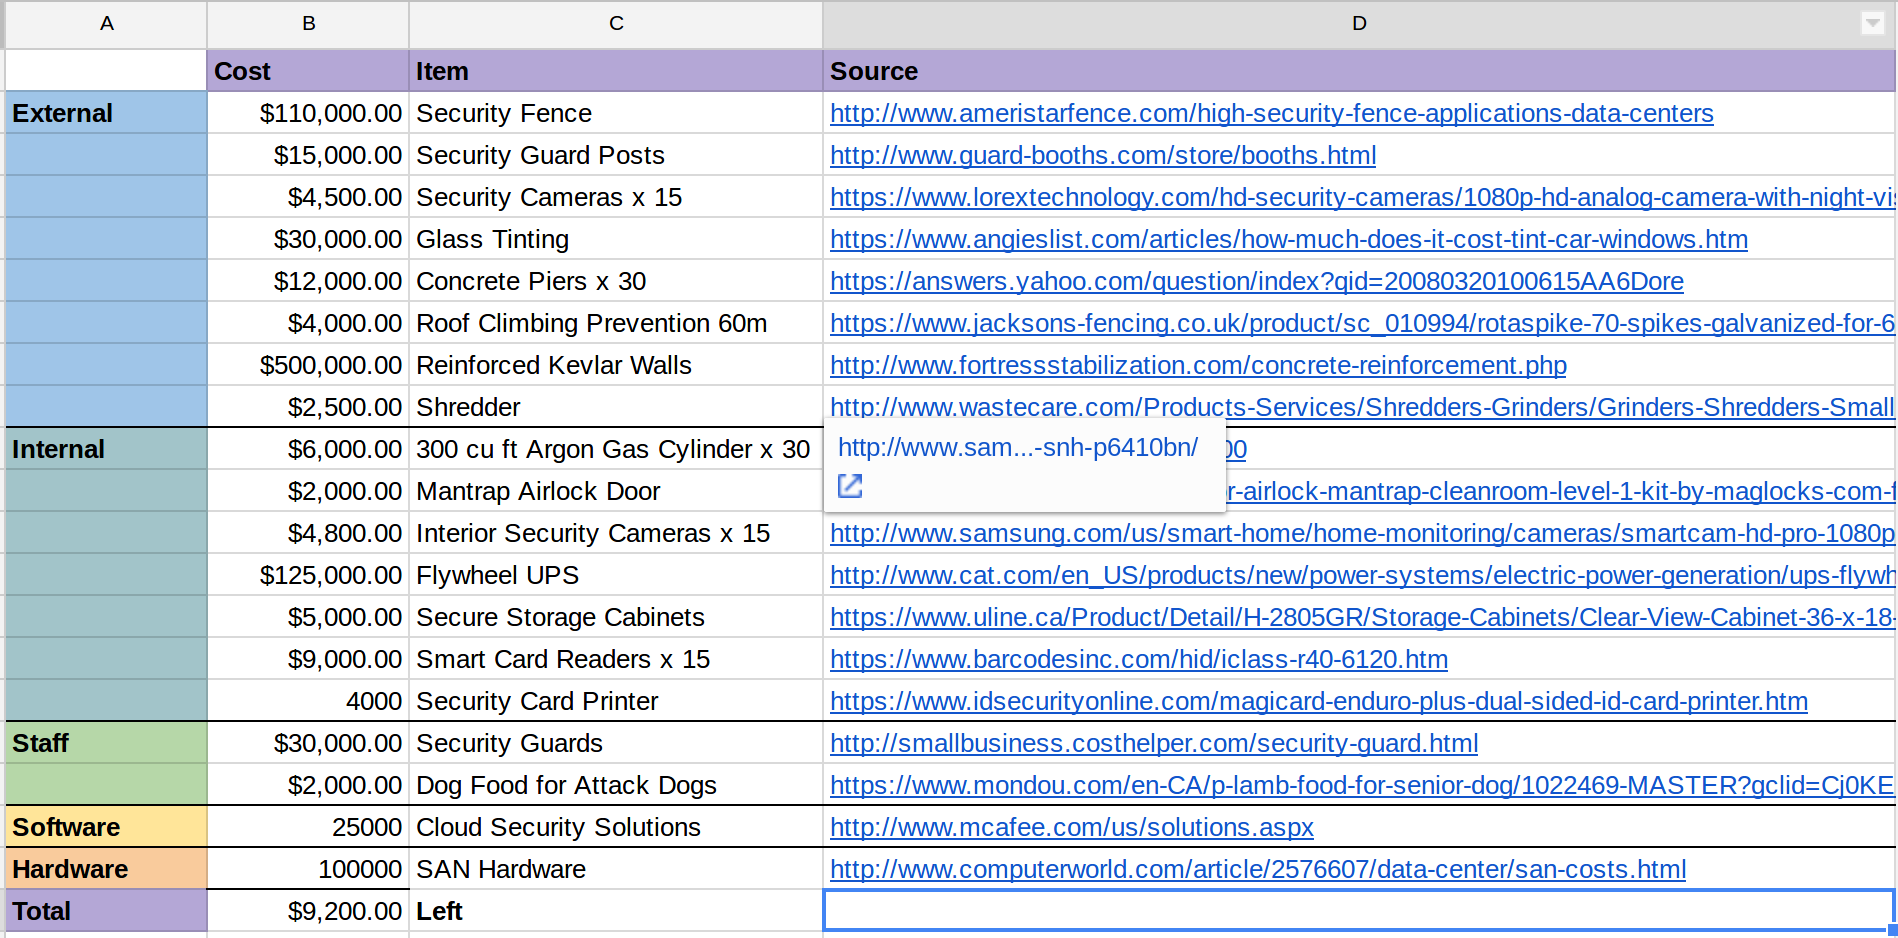
\includegraphics[scale=0.24]{budget.png}

I managed to have \$9200 dollars left over from the security budgetting.  Most items are difficult to find prices on as they all require quotes from the seller and there is little information on the prices.  Therefore on some of the prices I gave generous estimates.


\section*{Rationale}
In order to know what would be best for data center security, I used the follwing two sources: \href{https://www.unleashed-hosting.com/blog/2014/09/15/data-center-security-audit-checklist}{https://www.unleashed-hosting.com/blog/2014/09/15/data-center-security-audit-checklist} and \href{http://ptac.ed.gov/sites/default/files/ptac-data-security-checklist.pdf}{http://ptac.ed.gov/sites/default/files/ptac-data-security-checklist.pdf}.\\

The largest cost, as well as worry for securing a data center definitely seems to be on the outside perimeter.  If you can stop people from getting into the building to begin with, than everything inside will definitely be safe.  Therefore, for external security improvements we protected the perimeter by putting up large fences, anti-climbing deterants and concrete piers.  This makes sure that no one can easy walk in or drive through the walls of the building.  For people normally coming in and out we have security guard posts so there is a log of everyone entering and leaving and some form of a first-line of defense.  It is also important to have surveillance around the entire building, so I allocated enough money for 15 cameras to be used outside.  Lastly, we reinforce the walls with kevlar reinforced cement, making the walls even stronger, we also tint the windows so that the outside cannot easily see in and have an idea of the amount of assets we have.\\

Next, on hte inside we use airlock mantraps.  These, like the security gates, ensure that there is constant knowledge of who is inside the facilities, when and where.  These are just simple rooms with two doors on either side that requires a security guard to open the second door.  This brings up that we will need to hire security guards to protect the building as well, as well as guard dogs.  In the interior, we also have allocated for 15 cameras as this will monitor all of the equipment in the event that someone gets in.  These cameras have the potential to be shut off through a power outage, etc, therefore we have a flywheel UPS system to keep the important pieces of equipment running.  Card scanners will be used to gain access into various doors, and this will require a card printer.  In addition, there will be secure locked cabinets.\\

For software, we are going to go with Intel's security solutions by McAfee.  This is a cloud security solution and takes care of the issues of many things without it requiring an infrastructure cost to the company.  Also, we will require a hardware Storage Area Network to store and backup any files in the event of theft or failure.\\

For the most part, it is important to make sure the perimeter is secure and as this requires a lot of material and work it is the most costly aspect to securing any building including a data center.  Protecting a data center is not unlike many other secure buildings when it all boils down however.
%
%\begin{thebibliography}{9}
%\bibitem{Robotics} Fred G. Martin \emph{Robotics Explorations: A Hands-On Introduction to Engineering}. New Jersey: Prentice Hall.
%\bibitem{Flueck}  Flueck, Alexander J. 2005. \emph{ECE 100}[online]. Chicago: Illinois Institute of Technology, Electrical and Computer Engineering Department, 2005 [cited 30
%August 2005]. Available from World Wide Web: (http://www.ece.iit.edu/~flueck/ece100).
%\end{thebibliography}

\end{document}
